\chapter{Шугаман ба бусад хялбар хувиргалтууд}
\section{Ерөнхий шугаман функц}
 \subsection{Бүхэл шугаман функц}
 
\begin{eqnarray} \label{7.1}
W=az+b \ \ a\neq 0 (\text{үүнд:} a,b \ - \text{тогтмол комплекс тоонууд,)}
\end{eqnarray}
дүрстэй тавигдана. $\dfrac{1}{a}\neq 0$ тул (\ref{7.1})-ийн урвуу нь бас шугаман функц байна. $z=\infty$ байхад $w=\infty$ гэж урьдчилан тодорхойлолт хийж болох учир (\ref{7.1}) нь $\overline{\mathbb{C}}\rightarrow \overline{\mathbb{C}}$ харилцан нэгэн утгатай буулгана.

$a=|a|e^{i\alpha}$, $\alpha =\Arg  a$ байх тул $w=az+b=|a|e^{i\alpha}z+b$ болж бүхэл шугаман (\ref{7.1}) функц
\begin{enumerate}
    \item [$1^\circ$] $w_1=|a|z,$
     \item [$2^\circ$] $w_2=e^{i\alpha }w_1,$
      \item [$3^\circ$] $w=w_2+b$ гэсэн 3 хялбар буулгалтаар задлагдана.
\end{enumerate}
\begin{enumerate}
    \item [$1^\circ$]. $z$ цэгийг төвт төсөө (гомотет)-өөр $w_1$ цэгт буулгана. Энд төсөөгийн төв нь $z=0$, коэффициент нь $|a|$ байна (Зураг 26а).
    \begin{center}
    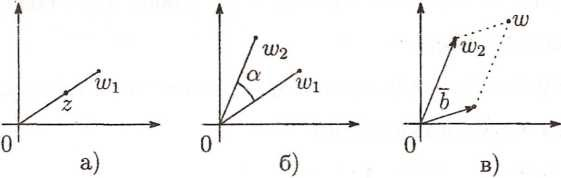
\includegraphics[width=8cm]{Zurag/26.jpg}
    \captionof{figure}{}
        \label{}
\end{center}
\item [$2^\circ$] $w_1=u_1+iv_1$, $w_2=u_2+iv_2$, $e^{i\alpha}=\cos \alpha +i\sin \alpha$ тус тус авбал 
$$
\begin{cases}
 u_2=u_1\cos \alpha-v_1\sin \alpha \\
 v_2=u_1 \sin \alpha +v_1\cos\alpha
\end{cases}
$$
болж $w_1$ нь $\alpha$ өнцгөөр эргэж $w_2$ цэгт бууна (Зураг 26б).
\item [$3^\circ$] $w=u+iv$, $w_2=u_2+iv_2$, $\overline{b}=b_1+ib_2$ гэж авбал
$$
\begin{cases}
 u=u_2+b_1 \\
 v=v_2+b_2
\end{cases}
$$ болж $w_2$ цэг өгөгдсөн тогтмол $\overline{b}$ вектортой параллель зөөлтөөр $w$ цэгт бууна (Зураг 26в).

Иймд бүхэл шугаман (\ref{7.1}) буулгалт нь дурдсан 3 хялбар буулгалтыг цувруулан гүйцэтгэсний үр дүн, өөрөөр хэлбэл, эдгээр буулгалтын үржвэрээр тодорхойлогдох болой.

Шугаман (\ref{7.1}) буулгалтыг 
\begin{eqnarray}
w-A=a(z-A)
\end{eqnarray}
байдалтай тавигдана гэвэл $A=\dfrac{b}{1-a}$ байна. $a=1$ бол ердийн параллель зөөлт.\\
$a\neq 0$ бол $A$-цэгийн орчинд эргүүлэхийг төсөөтэй буулгалттай хослуулан гүйцэтгэнэ.
\end{enumerate}
\begin{center}
    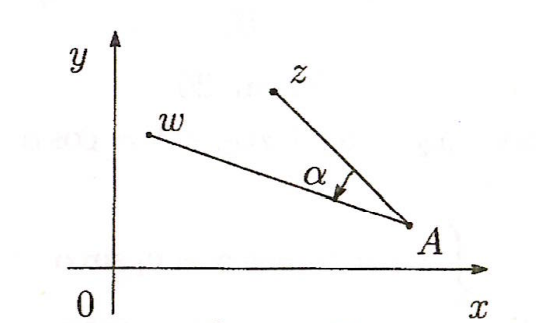
\includegraphics[width=6cm]{Zurag/27.PNG}
    \captionof{figure}{}
        \label{}
\end{center}
\section{Бутархай шугаман функц} \index{Бутархай шугаман функц}
\begin{eqnarray} \label{7.3}
w(z)=\frac{az+b}{cz+d}, \qquad ad-bc\neq 0
\end{eqnarray}
дүрстэй бичигдэх буулгалтыг бутархай шугаман функц \index{Шугаман функц} гэнэ. $a$, $b$, $c$, $d$-бэхлэгдсэн тогтмол комплекс тоонууд, $ad-bc\neq 0$ нь $w(z)$-ийн тогтмол тоо бишийг илтгэнэ. $(ad-bc=0$ байвал (\ref{7.3})-ын хүртвэр, хуваарь пропорциональ болж $w(z)$ нь $z$-ийн функц биш болоход хүргэнэ).

$c=0$, $d\neq 0$ тохиолдолд (\ref{7.3}) нь өмнө танилцсан бүхэл шугаман функц үүсгэнэ.

$c\neq 0$ үед (\ref{7.3}) нь $z\neq -\dfrac{d}{c}$, $\infty$ цэгүүд дээр тодорхойлогдоно. Харин онцгой $-\dfrac{d}{c}$ ба $\infty$ цэгүүд дээр $w(z)$-ийн тасралтгүй чанараар урьдчилан тодорхойлолт хийж $w\left(-\dfrac{d}{c}\right)=\infty$, $w(\infty)=\dfrac{a}{c}$ гэж авдаг.

$c=0$ үед шууд л $w(\infty)=\infty$ гэж авна.
\begin{thm}
(\ref{7.3}) нь $\overline{\mathbb{C}}$-г $\overline{\mathbb{C}}$-рүү гомеоморф (харилцан нэгэн утгатай, тасралтгүй) буулгана.
\end{thm}
\begin{prf}
$c=0$ үед илэрхий. $c\neq 0$ гэе. (\ref{7.3}) функц нийт $\overline{\mathbb{C}}$ дээр нэгэн утгатай тодорхойлогдоно. Нөгөөтээгүүр 
\begin{eqnarray} \label{7.4}
z=\frac{dw-b}{-cw+a}
\end{eqnarray}
өмнө тэмдэглэсэн урьдчилсан тодорхойлолт ёсоор $w=\dfrac{a}{c}$ цэгт $z=\infty$, харин $w=\infty$ цэгт $z=-\dfrac{d}{c}$ харгалзаж (\ref{7.3})-ийн $\overline{\mathbb{C}}$-г $\overline{\mathbb{C}}$- рүү харилцан нэгэн утгатай буулгах нь тогтоогдлоо. Одоо тасралтгүйг батлах үлдэв.

$z\neq -\dfrac{d}{c}$, $z\neq \infty$ үед (\ref{7.3}) тасралтгүй байх нь илэрхий. Харин эдгээр цэг дээр 
$$\lim\limits_{z\rightarrow -\frac{d}{c}}w(z)=\infty, \qquad \lim\limits_{z\rightarrow \infty} w(z)=\frac{a}{c}$$
хязгаарууд оршин байх тул мөн тасралтгүй. 
\hfill $\blacksquare$\end{prf}

Одоо бид, (\ref{7.3}) буулгалт $\overline{\mathbb{C}}$-ийн бүх цэг дээр өнцөг хадгалахыг батлан харуулъя. $z\neq -\dfrac{a}{c}$, $\infty$ цэгүүд дээр 
$$\frac{dw}{dz}=\frac{ad-cb}{(cz+d)^2}\neq 0$$
байх тул өнцөг хадгалагдана. Харин онцгой цэгүүдийн (хоёулаа төгсгөлгүйтэй холбоотой, нэг нь өөрөө төгсгөлгүй, нөгөөгийн дүр нь төгсгөлгүй) хувьд мөнхүү чанартайг тогтоохын тулд төгсгөлгүй цэг дээрх өнцгийн тухай ойлголт оруулъя.
\begin{dfn}
$z=\infty$ цэгийг дайрах замуудын (тэдгээр нь Риманы бөмбөрцгийн хойт туйл дээр огтлолцох шүргэгчүүдтэй) хооронд үүсэх өнцөг гэж
\begin{eqnarray}
Z=\dfrac{1}{z}
\end{eqnarray}
буулгалтын $Z=0$ дээрх $\Gamma_1$ ба $\Gamma_2$  дүрүүдийн хоорондох өнцгийг ойлгоно.
\end{dfn}
\begin{thm}
Бутархай шугаман (\ref{7.3}) буулгалт $\overline{\mathbb{C}}$-ийн цэг бүр дээр конформ буулгалт ($\infty$ дээр өнцөг хадгалагдах) өгнө.
\end{thm}
\begin{prf}
Онцгой биш цэгүүдийн хувьд теорем өмнө батлагдсан. $\gamma_1$ ба $\gamma_2$ нь $z=-\dfrac{d}{c}$ цэгийг дайрсан замууд бөгөөд энэ цэг дээр $\alpha$ өнцгөөр огтлолцсон байг. Эдгээр замын (\ref{7.3}) буулгалт дахь $w=\infty(z=-\dfrac{d}{c}$ цэгт харгалзах) цэг дээр $\gamma_1^*$ ба $\gamma_2^*$ дүрүүдийн хоорондох өнцөг нь тодорхойлолт ёсоор $\gamma_1^*$ ба $\gamma_2^*$-ийн $W=\dfrac{1}{w}$ буулгалт дахь $W=0$ цэг дээрх $\Gamma^*_1$ ба $\Gamma_1^*$ дүрүүдийн хоорондох өнцөгтэй тэнцүү. Харин
$$W=\frac{cz+d}{az+b}$$
бөгөөд иймд $\Gamma_1^*$ ба $\Gamma_2^*$ нь энэ буулгалт дахь $\gamma_1$ ба $\gamma_2$-ийн дүр.
$$\frac{dW}{dz}=\frac{bc-ad}{(az+b)^n}$$
уламжлал нь $z=-\dfrac{d}{c}$ цэг дээр $0$-ээс ялгаатай тул  $\Gamma_1^*$ ба $\Gamma_2^*$-ийн $W=0$ цэг дээр үүсгэх $\alpha$ өнцөгтэй тэнцүү. $z=-\dfrac{d}{c}$ цэгийн хувьд теорем батлагдлаа. $z=\infty$ цэгийн хувьд теоремыг батлахын тулд (\ref{7.3})-ийн урвуу (\ref{7.4}) функцэд өмнөх адил хандах явдал хүрэлцээтэй.
\hfill $\blacksquare$\end{prf}
\begin{thm}
Бутархай шугаман буулгалтуудын $\wedge$ цогц бүлэг үүсгэнэ.
\end{thm}
\begin{prf}
$$\zeta=\frac{a_1z+b_1}{c_1z+d_1} \ \ \text{ба }\ \ w=\frac{a_2\zeta+b_2}{c_2\zeta+d_2}$$
гэсэн бутархай шугаман хоёр буулгалт авч $\zeta$-ийн илэрхийллийг $w$-ийн томьёонд тавибал
$$w=\frac{az+b}{cz+d}$$ болж, энд
$$a=a_1a_2+d_2c_1 \qquad b=a_2b_1+b_2d_1$$
$$c=a_1c_2+c_1d_2 \qquad d=b_1c_2+d_1d_2$$
байх бөгөөд хэрэв $a_1d_1-b_1c_1\neq 0$ ба $a_2d_2-b_2c_2\neq 0$ байвал $ad-bc\neq 0$ байна.

Бид $L_1$,$L_2\in\wedge$ бол $L_1\circ L_2\in \wedge$ гэж баталлаа. \\
Одоо бүлгийн аксиомуудын биелэгдэхийг шалгая.
\begin{enumerate}
    \item [\textbf{a)}] 
    Дамжих чанар: $L_1$,$L_2$,$L_3\in \wedge$ бол
    \begin{eqnarray} \label{7.6}
    L_1\circ (L_2\circ L_3)=(L_1\circ L_2)\circ L_3
    \end{eqnarray}
    учир нь (\ref{7.6})-ийн хоёр тал $L_1(L_2[L_3(z)])$ гэж тавигдана.
    \item [\textbf{б)}] Нэгж буулгалт орших: нэгж нь адилтгал буулгалт болох нь мэдээж.
    \begin{eqnarray}
    \wedge \ni E:z\rightarrow z
    \end{eqnarray}
     \item [\textbf{в)}] Урвуу элемент орших: $\forall L\in\wedge$ байвал 
     \begin{eqnarray}
     L^{-1}\circ L=L\circ L^{-1}=E
     \end{eqnarray}
     байх $L^{-1}\in \wedge$ олдоно. Учир нь (\ref{7.3}) буулгалтын хувьд түүний урвуу элемент болох (\ref{7.4}) олдоно. 
\end{enumerate}
\hfill $\blacksquare$\end{prf}
\begin{hnt}
$\wedge$ бүлэг байр солих хуульд үл захирагдана.\\
Жишээ нь $L_1:z\rightarrow \dfrac{1}{z}$, $L_2:z\rightarrow z+1$ гэвэл $L_2\circ L_1:z\rightarrow \dfrac{1}{z}+1$, $L_1\circ L_2:\dfrac{1}{z+1}$
\end{hnt}
\begin{thm}
Аливаа бутархай шугаман буулгалт $\overline{\mathbb{C}}$ дээрх дурын тойргийг $\overline{\mathbb{C}}$ дээрх мөн л тойрогт хувиргана. (Үүнийг бутархай шугаман буулгалтын тойргийн чанар гэнэ).
\end{thm}
\begin{prf}
$c=0$ үед (\ref{7.3}) буулгалт $w=\dfrac{a}{d}z+\dfrac{b}{d}$ болж тойргийн төсөөтэй хувиргах, эргүүлэх ба параллель зөөлт хийхэд тойрог хэвээрээ байх билээ. Харин $c\neq 0$ 
\begin{eqnarray}
L:z\rightarrow \frac{az+b}{cz+d}=\dfrac{a}{c}-\frac{ad-bc}{c(cz+d)}=A+\frac{B}{z+C}
\end{eqnarray}
болж дараах гурван хялбар буулгалт
$$L_1:z\rightarrow A+Bz, \quad L_2:z\rightarrow \frac{1}{z}, \quad L_3:z\rightarrow z+C$$
гүйцэтгэсний дүнд $L$ хийгдэнэ $(L=L_1\circ L_2\circ L_3)$. Эхний ба эцсийн буулгалт $\overline{\mathbb{C}}$ дээр тойргийг хэвээр үлдээх нь мэдээж. $L_2:z\rightarrow \dfrac{1}{z}$ буулгалтын хувьд энэ чанар хэвээр хадгалагдахыг батлах л үлдлээ.

$\overline{\mathbb{C}}$ дээр аливаа тойргийн буюу шулууны тэгшитгэл, тэгш өнцөгт декартын координатын систем дээр 
\begin{equation} \label{7.10}
 A(x^2+y^2)+2D_1x+2E_1y+F=0   
\end{equation} 

дүрстэй тавигдана. Энд $A$, $D_1$, $E_1$, $F$ бодит тоонууд, харин $A$, $D_1$, $E_1$ нь нэгэн зэрэг тэгтэй тэнцэхгүй. Тухайлбал $A=0$ бол шулуун дүрсэлнэ. Харин $A_1\neq 0$ ба  $D_1^2+E_1^2>AF$ байвал тойрог. \z  гэж авбал \hz, $x^2+y^2=z\overline{z}$ ба \\ $2x=z+\overline{z}$, $2yi=z-\overline{z}$ болж эдгээрийг (\ref{7.10})-т тавихад шулуун буюу тойргийн комплекс хэлбэртэй
тэгшитгэл
\begin{eqnarray} \label{7.11}
Az\overline{z}+Dz+\overline{D}\overline{z}+F=0
\end{eqnarray}
бөгөөд энд $\overline{D}=D_1-E_1i$, $D=D_1+E_1 i.$

(\ref{7.11}) тойрог нь $L_2$ буулгалтаар ямар дүртэй болохыг мэдэхэд $z=\dfrac{1}{w}$, улмаар $\overline{z}=\dfrac{1}{\overline{w}}$ гэж орлуулах явдал хангалттай, иймд
\begin{eqnarray}
Fw\overline{w}+D\overline{w}+\overline{D}w+A=0
\end{eqnarray}
болж (\ref{7.10})-ийн адил тэгшитгэл гарлаа. Энэ нь $\mathbb{C}$ дээр мөн л тойрог дүрсэлнэ. 
\hfill $\blacksquare$\end{prf}

Одоо бутархай шугаман буулгалтын өөр нэг геометр чанартай танилцъя.
\begin{dfn}
\textbf{а). } Хэрэв $\Gamma =\{z:|z-z_0|=R\}$ тойргийн хувьд $z$ ба $z^*$ цэгүүд $z_0$-оос эхлэх цацраг дээр оршиж $z_0$ хүртэлх зайнуудын үржвэр $R^2$-тай тэнцэх: $(\arg  (z-z_0))=arg (z^*-z_0)$ ба $|z-z_0||z^*-z_0|=R^2$ байвал тэдгээрийг $\Gamma$ тойрогтой тэгш хэмтэй цэгүүд гэнэ.  \\
\textbf{б).} Эдгээр $z$, $z^*$ цэгүүдийг дайрсан $\overline{\mathbb{C}}$ дээрх аливаа тойрог $\Gamma$ тойрогтой ортогональ байвал \\
\begin{minipage}[b]{0.5\linewidth}
 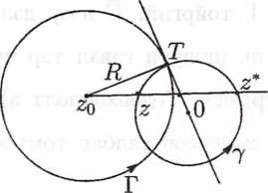
\includegraphics[width=5cm]{Zurag/28.jpg}
 \captionof{figure}{}
\end{minipage}
\hfill
\begin{minipage}[b]{0.5\linewidth}
    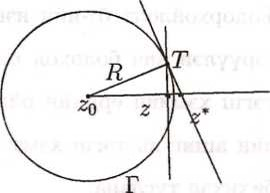
\includegraphics[width=5cm]{Zurag/29.jpg}
 \captionof{figure}{}
        \label{ref hiih ner}
\end{minipage}
\end{dfn}
Эдгээр тодорхойлолтын чацуу чанартай нь зураг 28-аас илэрхий. Хэрэв $z$, $z^*$ цэгүүд а) тодорхойлолт ёсоор $\Gamma$-тай тэгш хэмтэй бөгөөд $\gamma$ нь тэдгээрийг дайрсан аливаа тойрог байвал $z_0$ цэгээс $\gamma$-тойрогт татсан шүргэгчийн уртын квадрат нь элементар геометрийн теорем ёсоор огтлогч $|z_0-z^*|$ ба түүний гаднах хэсэг $|z_0-z|$-ийн үржвэртэй тэнцүү.

Иймд $z_0$ цэгээс $\gamma$-д татсан шүргэгч нь $\Gamma$-ийн радиус байх тул энэ тойргууд ортогональ. (Хэрэв $\gamma$ нь шулуун ч байсан тэр нь $z_0$-ийг дайрах учир $\Gamma$-тай ортогональ). Урвуугаар, $\overline{\mathbb{C}}$ дээр орших $z$ ба $z^*$ цэгүүдийг дайрсан аливаа $\gamma$-тойрог (тухайн тохиолдлын $zz^*$-шулуун) $\Gamma$-д ортогональ байвал нэгдүгээрт, $z$ ба $z^*$ цэгүүд $z_0$-оос эхлэх цацраг дээр орших бөгөөд хоёрдугаарт, тэдгээрээс $z_0$ хүртэлх зайнуудын үржвэр $R^2$-тай тэнцүү (элементар геометрийн мөнхүү теорем ёсоор) иймд $z$ ба $z^*$ цэгүүд  $\Gamma$-тай тэгш хэмтэй байна.

Тодорхойлолт б)-ийн нэг ашиг нь $\Gamma$ тойргийг $\overline{\mathbb{C}}$ дээр дэлгэрүүлэн авч болоход оршино: $\Gamma$ нь шулуун гэвэл тэр нь тэгш хэмийн ердийн ойлголтод хүргэнэ. Тодорхойлолт а)- ийн ашиг нь тэгш хэмт цэгүүдийг холбосон хялбар томьёо бичихэд тусална:
$$arg(z^*-z_0)=arg(z-z_0) \ \ \text{ба} \ \ |z-z_0|\cdot |z^*-z_0|=R^2$$
нөхцөлүүдээс
\begin{eqnarray} \label{7.13}
z^*=z_0+\frac{R^2}{\overline{ z-z_0}}
\end{eqnarray}
томьёо гарна. 

Зураг 29, тэгш хэмт цэгүүдийг хэрхэн байгуулахыг заана: $z$ нь $\Gamma$ дотор байвал $z$-ээс $z_0z$ цацрагт перпендикуляр татаж тойрогтой огтлолцох $T$ цэг олж $T$-ээс $\Gamma$-д татсан шүргэгчийн цацрагтай огтлолцоход $z^*$ цэг олдоно.

Хэрэв $z$ нь $\Gamma$-ийн гадаа байвал байгуулалт урвуу эрэмбээр хийгдэнэ (Баталгаа нь $z_0zT$ ба $z_0Tz^*$ гурвалжнуудын төсөөгөөс үүдэн гарна).

$z\in \overline{\mathbb{C}}$ цэг бүрийг $\Gamma$ тойргийн түүнтэй тэгш хэмтэй $z^*$ цэгт буулгах $z\rightarrow z^*$ буулгалтыг энэ тойрогтой харьцуулсан тэгш хэм буюу инверси \index{Инверси} гэж нэрлэнэ.

(\ref{7.13})-аас харахад $\overline{\mathbb{C}}$ дээрх тойрогтой харьцуулсан инверси нь бутархай шугаман функцийн хосмог функцээр илэрхийлэгдэнэ.

Одоо тэгш хэмт цэгүүдийн хадгалагдах чанарыг харуулсан дараах теоремтой танилцъя.

\begin{thm}
Аливаа бутархай шугаман $L$ буулгалт $\overline{\mathbb{C}}$ дээрх ямар нэгэн $\Gamma$ тойрогтой харьцуулсан тэгш хэмт дурын $z$ ба $z^*$ цэгүүдийг энэ тойргийн $L(\Gamma)$ дүртэй харьцуулсан тэгш хэмт $w$ ба $w^*$ цэгүүдэд хувиргана (тэгш хэмт цэгүүдийн хадгалагдах чанар).
\end{thm}
\begin{prf}
$z$ ба $z^*$ цэгүүдийг дайрах $\overline{\mathbb{C}}$ дээрх $\Gamma$ тойрогт ортогональ бүхий л тойргуудын бүлийг $\{\gamma\}$ гэж тэмдэглэе.

Теорем 7.1 ёсоор $\gamma$ тойргууд $\overline{\mathbb{C}}$ дээрх $L(\gamma)$ тойргуудад буух бөгөөд харин $L$-ийн конформлог чанараар бүх $L(\gamma)$ тойргууд $L(\Gamma)$-д ортогональ байна. Эндээс бүх $L(\gamma)$ тойргуудын дайрах $w$ ба $w^*$ цэгүүд $L(\Gamma)$-тай харьцуулсан тэгш хэмт байх нь тогтоогдов. 
\hfill $\blacksquare$\end{prf}
\section{Бутархай шугаман изоморфизм ба автоморфизм}
Бутархай шугаман буулгалтын
\begin{eqnarray}
L:w=\frac{az+b}{cz+d}
\end{eqnarray}
томьёонд $a$, $b$, $c$, $d$ гэсэн дөрвөн комплекс коэффициент орох боловч түүнийг гурван комплекс параметрээс хамаарах мэт үндэс байна. Учир нь бутархайн хүртвэр ба хуваарийг $0$-ээс ялгаатай аль $1$ коэффициентод хувааж болно. Үүнийг ашигласны дүнд дараах теорем батлагдана.
\begin{thm}
Аливаа ялгаатай $3$-н $z_1$, $z_2$, $z_3\in\mathbb{C}$ цэг ба мөнхүү ялгаатай $3$-н $w_1, w_2, w_3\in\mathbb{C}$ цэг авахад $L(z_k)=w_k$, $k=1,2,3$ байх бутархай шугаман $L$ буулгалт олдох ба тэр нь цор ганц.
\end{thm}
\begin{prf}
Тийм $L$ буулгалт оршин байх нь хялбархан батлагдана: $z_k$ ба $w_k(k=1,2,3)$ цэгүүдийг харгалзан $\zeta$ хавтгайн $0,\infty,1$ цэгүүдэд буулгах бутархай шугаман $L_1$ ба $L_2$ буулгалт байгуулъя:
\begin{eqnarray} \label{7.15}
L_1:\zeta=\frac{z-z_1}{z-z_2}\cdot \frac{z_3-z_2}{z_3-z_1}, \quad
L_2:\zeta=\frac{w-w_1}{w-w_2}\cdot \frac{w_3-w_2}{w_3-w_1}
\end{eqnarray}
гэвэл 
\begin{eqnarray} \label{7.16}
L=L^{-1}_2 \cdot L_1
\end{eqnarray} буулгалт
\begin{eqnarray} \label{7.17}
\frac{z-z_1}{z-z_2}\cdot \frac{z_3-z_2}{z_3-z_1}=\frac{w-w_1}{w-w_2}\cdot \frac{w_3-w_2}{w_3-w_1}
\end{eqnarray}
шүтэлцэл $w=w(z)$ функц тодорхойлох ба тэр нь бидний эрж буй функц. Учир нь (\ref{7.17})-бутархай шугаман функц байхын хамт $z_k$-ийг $w_k$-д $(k=1,2,3)$ буулгах нь илэрхий.

Одоо буулгалтын цор ганц байхыг баталъя.

$\lambda$ нь $\lambda(z_k)=w_k \quad (k=1,2,3)$ байх ямар нэг бутархай шугаман буулгалт байг. (\ref{7.15}) томьёогоор тодорхойлогдох $L_1$ ба $L_2$-ийн хувьд $\mu =L_1\circ \lambda\circ L_1^{-1}$ буулгалт авбал тэр нь $0,\infty, 1$ цэгүүдийг үл хөдөлгөх нь ойлгомжтой. $\mu (\infty)=\infty$ нөхцөлөөс $\mu$ нь бүхэл шугаман функц: $\mu(\zeta)=\alpha\zeta +\beta$, $\mu(0)=0$ нөхцөлөөс $\beta =0$ ба $\mu(1)=1$ нөхцөлөөс $\alpha =1$ . Иймд $\mu\zeta =\zeta$ бөгөөд өөрөөр хэлбэл $L_2\cdot \lambda \cdot L_1^{-1}=E$ болох тул $\lambda =L_2^{-1}\cdot L_1$ буюу (\ref{7.16}) ёсоор $\lambda =L.$
\hfill $\blacksquare$\end{prf}
\begin{hnt}
$z_k$ ба $w_k$ цэг бүр (\ref{7.17}) шүтэлцэлд хоёр удаа орохдоо нэг удаа хүртвэрт, нөгөө удаа хуваарьт байх тул $z_k$ буюу $z_k$-ийн аль нэг нь $\infty$ байхад (\ref{7.17}) нь хүчинтэй байна. Бутархайн хүртвэр ба хуваарийн хаана нь $\infty$ тавигдана түүнийг 1-ээр солих хэрэгтэй. Жишээ нь $z_1=w_2=\infty$ байвал 
$$\frac{1}{z-z_2}\cdot \frac{z_3-z_2}{1}=\frac{w-w_1}{w-w_2}\cdot \frac{1}{1}$$

(\ref{7.17}) тэгшитгэлээс бутархай шугаман хувиргалтын бас нэг ерөнхий чухал чанар батлагдана. $a$, $b$, $c$, $d$ нь хоорондоо ялгаатай (төгсгөлгүй) дурын комплекс тоонууд байг.
$$\frac{c-a}{c-b}:\frac{d-a}{d-b}$$
гэсэн харьцаануудын харьцааг $a$, $b$, $c$, $d$ дөрвөн тооны буюу цэгийн (ангармоник буюу) давхар харьцаа \index{Ангармоник буюу) давхар харьцаа} гэж нэрлэнэ. Энэ харьцааг ($a$, $b$, $c$, $d$) гэж тэмдэглэх бөгөөд
$$(a,b,c,d)=\frac{c-a}{c-b}:\frac{d-a}{d-b}$$
юм.

Давхар харьцааны дээрх тодорхойлолтыг эдгээр $4$ цэгийн аль нэг нь $\infty$ байх тохиолдолд өргөтгөж болно. Дотор нь төгсгөлгүй алсын цэг багтах $4$ цэгийн давхар харьцаа гэж $3$ нь өгөгдсөн цэгүүдтэй таарах, $4$ дэх нь $\infty$ рүү тэмүүлэх хязгаарын утгыг нэрлэнэ. Энэ тодорхойлолт ёсоор
$$(\infty, b,c,d)=\frac{1}{c-b}:\frac{1}{d-b}$$
$$(a,\infty, c, d)=(c-a):(d-a)$$
$$(a,b,\infty, d)=1:\frac{d-a}{d-b}$$
$$(a,b,c,\infty) =\frac{c-a}{c-b}$$
байна.

Бутархай шугаман $w=w(z)$ функц хоорондоо ялгаатай $a$, $b$, $c$, $d$ $4$ цэгийг $A$, $B$, $C$, $D$ $4$ цэгт буулгадаг. 
\end{hnt}
\begin{thm}
Аливаа бутархай шугаман буулгалт $4$ цэгийн давхар харьцааг үл өөрчилнө:
$$(a,b,c,d)=(A,B,C,D)$$
Өөрөөр хэлбэл, $4$ цэгийн давхар харьцаа нь бутархай шугаман буулгалтын инвариант чанар юм. Теорем 7.1 болон тойргийн чанарыг үндэслэн $\overline{\mathbb{C}}$ дээрх аливаа $\Gamma$ тойргийг бутархай шугаман буулгалтаар аливаа өөр  $\Gamma^*$ тойрогт хувиргаж болно (Ингэхдээ $\Gamma$ тойргийн $3$ цэгийг $\Gamma^*$ тойргийн $3$ цэгт буулгаад тойргийн чанар ашиглах явдал л хангалттай). Топологи ухааралтын үүднээс $\Gamma$-аар зааглагдсан $B$ дугуй $\Gamma^*$-аар зааглагдсан хоёр дугуйн нэгэнд (чухамхүү алинд нь буухыг ямар нэгэн $z_0\in B$ цэг хаана бууж байгаагаар мэднэ) буух нь мэдээж.

Эндээс ямар нэгэн $B\subset \overline{\mathbb{C}}$ дугуй бутархай шугаман хувиргалтаар ямар нэгэн өөр  $B^*\subset \overline{\mathbb{C}}$ дугуйд буух нь ч ойлгомжтой болов.

$D$ мужийг $D^*$ мужид буулгах бутархай шугаман буулгалтыг бутархай шугаман изоморфизм гэх ба $D$ ба $D^*$ мужуудын хувьд тийм изоморфизм оршин байвал тэдгээрийг бутархай шугаман изоморф \index{Изоморфизм} гэнэ.

Дөнгөж саяхан нотломжлон хэлсэн өгүүлбэрийг теорем байдлаар томьёолж болно.
\end{thm}
\begin{thm}
$\overline{\mathbb{C}}$ дахь аливаа $2$ дугуй бутархай шугаман изоморф.

Одоо жишээ болгож дээд хагас хавтгай $(\im z>0)$-ийг нэгж $(|w|<1)$ дугуйд буулгах бүхий л тийм изоморфизм олъё. Үүний тулд $a$, $\im a>0$ цэг бэхлэн авч түүнийг $|w|<1$ дугуйн төвд буулгасан гэж бодъё. Тэгвэл $a$-тай бодит тэнхлэгийн хувьд тэгш хэмтэй $\overline{a}$ цэг өмнөх зүйлийн теорем 7.5 ёсоор $|w|=1$ тойргийн хувьд $w=0$ цэгтэй тэгш хэмтэй $w=\infty$ цэгт бууна. Иймд эдгээр цэгийг $0$ ба $\infty$-д харгалзан буулгах бутархай шугаман (тогтмол $k$ үржигдэхүүний нарийвчлалтайгаар) буулгалт
$$w=k\cdot \frac{z-a}{z-\overline{a}}$$
дүрстэй тавигдана.

Бодит $z=x$ үед $|z-a|=|z-\overline{a}|$ тэнхлэг нэгж тойрогт буухын тулд $|k|=1$ гэж авах хэрэгтэй. Өөрөөр хэлбэл $k=e^{i\theta}$. Иймд дээд хагас хавтгай $(\im z>0)$ нэгж дугуй $(|w|<1)$-д буулгах бутархай шугаман изоморфизмүүд 
\begin{eqnarray} \label{7.18}
w=e^{i\theta}\cdot \frac{z-a}{z-\overline{a}}
\end{eqnarray}
томьёогоор тодорхойлогдоно. ($a$ дээд хагас хавтгайн аливаа цэг, $\theta$-бодит тоо)

Мужийг өөрт нь буулгадаг бутархай шугаман изоморфизмыг бутархай шугаман автоморфизм\index{Автоморфизм} гэнэ. Ямар нэгэн бутархай шугаман бүх автоморфизмүүдийн бөөгнөрөл бутархай шугаман буулгалтуудын $\wedge$-бүлгийн дэд бүлэг үүсгэх нь ойлгомжтой.

$\overline{\mathbb{C}}$-г $\overline{\mathbb{C}}$-рүү буулгах бүх бутархай шугаман автоморфизмүүдийн бөөгнөрөл $\wedge$ бүлэгтэй давхацна. $\mathbb{C}$-г $\mathbb{C}$-рүү буулгах бутархай шугаман автоморфизмүүдийн бөөгнөрөл $z\rightarrow az+b$, $a\neq 0$ гэж буулгах бүхэл шугаман хувиргалтуудын дэд $\wedge_0$ бүлэгтэй давхцах нь ч бас мэдээж. Одоо нэгж дугуйн автоморфизмүүдийн бүлгийг бодож гаргая. Тойргийн төв $w=0$ цэгт буух $a$, $|a|<1$ цэгийг бэхлэн авъя. $a$-цэгтэй нэгж тойргийн $\{|w|<1\}$ хувьд тэгш хэмтэй $a^*=\dfrac{1}{\overline{a}}$ цэг $w=\infty$ цэгт буух учиртай. Иймд бидний эрж буй буулгалт
$$w=k\cdot \frac{z-a}{z-\frac{1}{\overline{a}}}=k_1\cdot \frac{z-a}{1-\overline{a}\cdot z}$$
дүрстэй ($k$, $k_1$ нь тогтмол) бичигдэнэ. $z=1$ цэг нэгж тойргийн цэгт буух тул $|k_1|\cdot \left|\frac{1-a}{1-\overline{a}}\right|=|k_1|=1$ болно. Өөрөөр хэлбэл, $k_1=e^{i\theta}$, $\theta$-бодит тоо. Иймд нэгж дугуйн автоморфизм
\begin{eqnarray}
w=e^{i\theta}\frac{z-a}{1-\overline{a}z}
\end{eqnarray} болой.
\end{thm}
\section{Зарим рациональ функц}
\subsection{Зэрэгт функц\index{Зэрэгт функц}}

Натурал $n$ тооны хувьд $\mathbb{C}$ дээр голоморф
\begin{eqnarray} \label{7.20}
w=z^n
\end{eqnarray}
функцийг зэрэгт функц гэнэ. Түүний уламжлал
$\dfrac{dw}{dz}=nz^{n-1}$, $(n>1)$ нь  $z\neq 0$ үед $0$-ээс ялгаатай тул
$z\in\mathbb{C}\setminus \{0\}$ цэг бүр дээр конформ буулгалт өгнө.

Зэрэгт функц $0$ цэгийн орчинд ямар төрхтэй байхыг авч үзье. Үүний тулд туйлын координат:
$$z=re^{i\varphi}, \qquad w=\rho e^{i\theta}$$
ашиглавал (\ref{7.20}) тэнцлээр
\begin{eqnarray} \label{7.21}
\begin{cases}
 \rho=r^n \\
 \theta =n\varphi
\end{cases}
\end{eqnarray}
болно. (\ref{7.21})-ийн $2$дугаархаас өнцөг $0$ цэг дээр хэвээр хадгалагдахгүй, харин $n$ дахин өсөх нь тодорхой байна. Өнцгийн хадгалагдах чанаргүй байх нь $\infty$ дээр ч мөн адил. Учир нь $\dfrac{1}{w\left(\frac{1}{z}\right)}$ функц  $z=0$ цэгийн орчинд өгөгдсөн функцтэй давхацна.

$0$ ба $\infty$ цэг нь $z=\sqrt[n]{w}$ функцийн салаалалтын цэгүүд болдог. (\ref{7.21})-ээс харахад $\circled{z}$ хавтгайн $0$ цэгт төвтэй тойрог \\ $(r=const)$ $\circled{w}$ хавтгай $(\rho =consrt)$-т, $0$ цэгээс гарсан цацраг ($\varphi=const$) мөн цацраг ($\theta =const$)-т буух нь тодорхой байна.

$\circled{z}$ хавтгай дээр бодит эерэг тэнхлэг ба $0$ цэгээс гарсан цацрагаар үүсгэгдсэн $\dfrac{2\pi}{n}$ өнцөгт харгалзах сектор (зураг 30) авъя. Энэ сектор (\ref{7.20}) функцээр $\circled{w}$ хавтгайн эерэг хагас тэнхлэгийн дагуу хагалбар бүхий бүх хавтгай (зураг 31)-д бууна. Учир нь $\varphi =0$ бол $\theta =0$, $\varphi =\dfrac{2\pi}{n}$ бол $\theta =2\pi $ өнцөг харгалзана. \\
\begin{minipage}[b]{0.5\linewidth}
 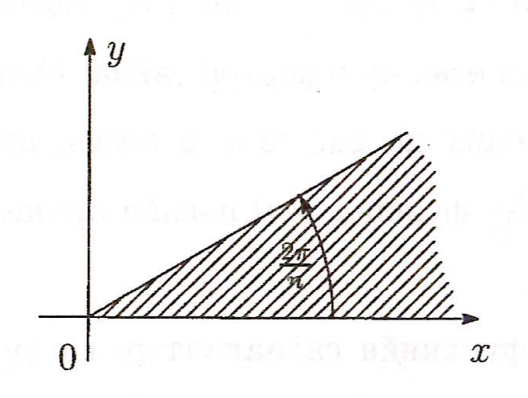
\includegraphics[width=5cm]{Zurag/30.PNG}
 \captionof{figure}{}
\end{minipage}
\hfill
\begin{minipage}[b]{0.5\linewidth}
    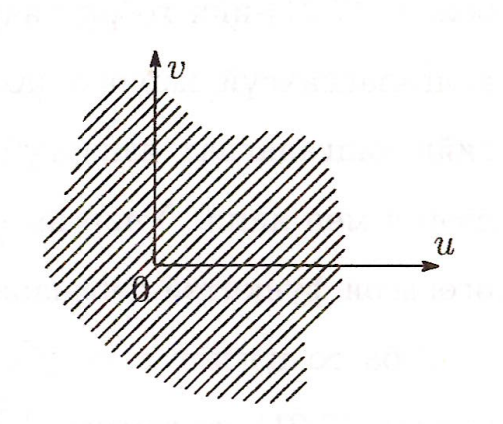
\includegraphics[width=5cm]{Zurag/31.PNG}
 \captionof{figure}{}
        \label{ref hiih ner}
\end{minipage}
Өөрөөр хэлбэл (\ref{7.20}) функц $D=\left\{0<\arg  z<\dfrac{2 \pi}{n}\right\}$ секторийг
$D^*=\{0< \arg  w<2 \pi \}$ мужид гомеоморф буулгана.
\subsection{Жуковскийн функц.} \index{Жуковскийн функц}
$\mathbb{C}\setminus \{0 \}$ мужид голоморф
\begin{eqnarray} \label{7.22}
w=\frac{1}{2}\left(z+\frac{1}{z}\right)
\end{eqnarray}
рационал функцийг Жуковскийн функц гэнэ. Түүний хувьд
$$\frac{dw}{dz}=\frac{1}{2}\left(1-\frac{1}{z^2}\right)$$ 
бөгөөд $z\neq \pm 1$ цэг дээр $0$ ялгаатай тул (\ref{7.22}) функц $z\neq 0$, $\pm 1$ цэг бүр дээр конформ буулгалт өгнө. 

Ямар нэг $D$ муж дээр манай функцийн нэг хуудаст байх нөхцөлийг тогтооё. Энэ функц $z_1$, $z_2$ цэгийг нэгэн цэгт буулгалаа гэвэл
$$z_1+\frac{1}{z_1}-\left(z_2+\frac{1}{z_2}\right) =(z_1-z_2)\left(1-\frac{1}{z_1z_2}\right)=0$$
байх учиртай бөгөөд $z_1\neq z_2$ бол $z_1z_2=1$ байх аж. Иймд
Жуковскийн функц ямар нэг $D$ муж дээр нэг хуудаст байх зайлшгүй бөгөөд хүрэлцээтэй нөхцөл нь
\begin{eqnarray}
z_1\cdot z_2=1
\end{eqnarray}
гэсэн ямар ч хос $D$-мужид агуулагдахгүй байх явдал мөн.

Нэг хуудаст мужийн жишээ нь нэгж дугуйн гаднах хэсэг $D=\{z\in\overline{\mathbb{C}}\}:|z|>1$ юм. (\ref{7.22}) буулгалтыг ил харуулахын үүднээс $z=re^{i\varphi}$, $w=u+iv$ гэж авбал (\ref{7.22}) 
\begin{eqnarray}
u=\frac{1}{2}\left(r+\frac{1}{r}\right) \cos \varphi, \qquad v=\frac{1}{2}\left(r-\frac{1}{r}\right) \sin \varphi
\end{eqnarray}
дүрстэй бичигдэнэ.

Эдгээр шүтэлцлээс Жуковскийн функц $\{|z_1|<r_0\}, r_0>1$ байх аливаа тойрог $a_{r_0}=\dfrac{1}{2}\left(r_0+\dfrac{1}{r_0}\right)$ ба $b_{r_0}=\dfrac{1}{2}\left(r_0-\dfrac{1}{r_0}\right)$ гэсэн хагас тэнхлэгүүд бүхий $\pm 1$ цэгүүдэд фокустай ($\forall r_0$- ийн хувьд $a^2_{r0}-b_{r0}^2=1$ тул) эллипст буух нь харагдаж байна (зураг 23 үз). \\
\begin{center}
    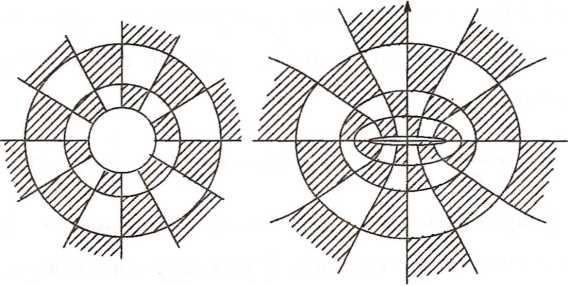
\includegraphics[width=7cm]{Zurag/32.jpg}
    \captionof{figure}{}
        \label{}
\end{center}
$\lim\limits_{r_0\rightarrow 1} b_{r_0}=0$ байх тул эллипс $[-1;1]\subset \mathbb{R}$ хэрчим рүү унтрана. $a_{r_0}-b_{r_0}$ ялгавар $\dfrac{1}{r_0}$ болж их хэмжээний $r_0$-ийн хувьд эллипс нь тойргоос багаар ялгагдана.

$\{\varphi =\varphi_0$, $1<r<\infty\}$ цацраг $\dfrac{u^2}{\cos\varphi}-\dfrac{v^2}{\sin^2\varphi}=1$ гиперболын хэсэгт буух ба мөн  $\pm 1$ цэгүүдэд фокустай ($\forall \varphi_0$-ийн хувьд $\cos^2_0+\sin^2\varphi_0=1$ тул) зураг 32-г үз.

Конформ чанараар эдгээр гиперболын бүл уул эллипсүүдийн бүлтэй ортогональ.

Дээр дурдсанаас харахад Жуковскийн функц нэгж тойргийн гаднах (төгсгөлгүй алсын цэгийг агуулах) хэсгийг бодит тэнхлэгийн $[-1;1]$ хэрчмийн гаднах хэсэгт харилцан нэгэн утгатай, конформ буулгах нь илэрхий болов.

$\pm 1$ цэгүүдэд (\ref{7.22}) буулгалт конформ биш. Үүнд үнэмшихийн тулд Жуковскийн функцийг
\begin{eqnarray} \label{7.25}
\frac{w-1}{w+1}=\left(\frac{z-1}{z+1}\right)^2
\end{eqnarray}
дүрстэй бичье. (\ref{7.25})-ийг
\begin{eqnarray} \label{7.26}
\zeta =\frac{z-1}{z+1}, \quad w=\zeta^2,\quad w=\frac{1+w}{1-w}
\end{eqnarray}
байдалтай бичиж (сүүлчийнх нь $w=\dfrac{w-1}{w+1}$-ийн урвуу) болно. (\ref{7.26})-ийн эхнийх ба гуравдах нь бутархай шугаман тул нийт $\overline{\mathbb{C}}$ дээр конформ буулгалт өгнө. Харин $w=\zeta ^ 2$ буулгалт $\zeta =0$, $\infty$ цэгүүдэд ($z=\pm 1$) дээрх өнцгийг хоёр дахин өсгөнө.

(\ref{7.25}) задаргаанаас Жуковскийн функц зураг 24-т үзүүлсэнчлэн ($\pm 1$ цэгүүдийг дайрахдаа бодит тэнхлэгтэй $\alpha$ өнцөг үүсгэх) $\gamma$-тойргийн гаднах хэсгий тойргийн нумын ($\pm 1$ цэгүүдэд төгсгөл бүхий бодит тэнхлэгтэй $w=1$ цэг дээр $2\alpha$ өнцөг үүсгэх) гаднах хэсэгт нэг хуудаст бөгөөд конформ буулгах нь илт байна.

Мөн энэ буулгалтаар $\gamma$ тойрогтой $\pm 1$ цэгүүдийн аль нэг дээр гадаад шүргэх $\delta$-тойргийг нисэх онгоцны далавчны хөндлөн огтлол санагдуулах өвөрмөц битүү $\delta '$ муруйд буух (зураг 33-г үз) нь харагдаж байна. \\
\begin{center}
    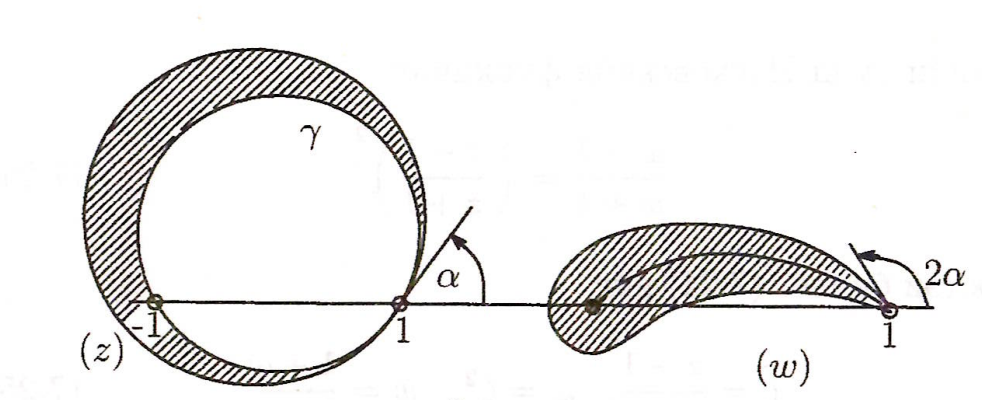
\includegraphics[width=8cm]{Zurag/33.PNG}
    \captionof{figure}{}
        \label{}
\end{center}
Энэ санамж далавчны аэродинамик тооцооны анхны аргыг боловсруулахад нь Жуковскийд тусалжээ.
\section{Зарим трансцендент функц, түүний буулгалт}
\subsection{Илтгэгч функц \index{Илтгэгч функц, (экспонент)} тодорхойлох нь.}
$\dfrac{df}{dz}=f(z)$ ба $f(0)=u(0,0)+iv(0,0)=1$ нөхцөлүүд хангах голоморф функц олъё. 
$$\frac{df}{dz}=\frac{\partial u}{\partial x}+i\frac{\partial v}{\partial x}=\frac{\partial v}{\partial y}-i\frac{\partial u}{\partial y}$$ 
байх тул манай дифференциал тэгшитгэл
$$\frac{\partial u}{\partial x}+i\frac{\partial v}{\partial x}=\frac{\partial u}{\partial y}-i\frac{\partial u}{\partial y}= u+iv$$
дүрстэй болж эндээс
$$\frac{\partial u}{\partial x}=\frac{\partial v}{\partial y}=u,\qquad \frac{\partial v}{\partial x}=-\frac{\partial u}{\partial y}= v$$
бөгөөд $\dfrac{\partial u}{\partial x}=u$ ба $u(0,0)=1$ нөхцөлөөс $u(x,y)=e^x\lambda (y)$ болно. (Энд $\lambda (y)$ нь $\lambda(0)=1$ нөхцөл хангах дифференциалчлагдах функц.) Яг энэчлэн $\dfrac{\partial v}{\partial x}=v$ ба $u(0,0)=0$ нөхцөлөөс $v(x,y)=e^x\cdot \mu (y)$ болно. (энд $\mu(y)$ нь $\mu(0)=0$ нөхцөл хангах дифференциалчлагдах функц.) Иймд
$$\frac{\partial v}{\partial y}=e^x \mu'(y)=u=e^x\lambda(y), \qquad -\frac{\partial u}{\partial y}=-e^x \lambda'(y)=v=e^x\mu(y). $$
Өөрөөр хэлбэл
$$\mu'(y)=\lambda (y), \qquad -\lambda '(y)=\mu (y).$$
Эндээс $\lambda(y)$ ба $\mu(y)$ функцүүд ерөнхий шийд нь
$$\varphi (y)=c_1\cos y+c_2\sin y$$
байх хоёрдугаар эрэмбийн шугаман дифференциал
$$\frac{d^2\varphi(y)}{dy^2}+\varphi (y)=0$$
тэгшитгэлийг хангах нь мэдээж юм. $\mu (y)$-ийн анхны нөхцөлийг тооцвол $\mu(y)=C\sin y$ болж улмаар $\lambda (y)=\mu '(y)=C\cos y$ бөгөөд эндээс $C=1$-ийн анхны нөхцөл ёсоор $\lambda(y)=\cos y$, $\mu (y)=\sin y$ болно.

Иймд  $\lambda (y)=\cos y$, $\mu(y)=\sin y$ эндээс
$$f(z)=u(x,y)+iv(x,y)=e^x(\cos y +i\sin y)$$ болов. 

Бид дурдсан нөхцөлүүд хангах цор ганц голоморф функц оллоо.

Энэ функцийг комплекс $z$ хувьсагчийн экспонент буюу илтгэгч функц гэх ба $\exp z$ гэж тэмдэглэнэ:
\begin{eqnarray} \label{7.27}
\exp z=e^z=e^x(\cos y +i\sin y)
\end{eqnarray}
Эндээс 
\begin{eqnarray}
|e^z|=e^{\re z}, \qquad \arg  e^z=\im z
\end{eqnarray}
бөгөөд (\ref{7.27})-д $z=0$ байвал Эйлерийн\index{Эйлерийн томьёо }
\begin{eqnarray}
e^{iy}=\cos y +i\sin y
\end{eqnarray}
томьёо батлагдлаа.

I бүлэгт $e^{iy}$ гэдгийг баруун $pq$ илэрхийллийн товчилсон тэмдэглэгээ төдий хэрэглэсэн бол одоо түүнийг $e$-ийн хуурмаг зэрэг гэж ойлгох боломж бидэнд олдлоо.

Илтгэгч функцийн үндсэн чанаруудыг тоочъё:
\begin{enumerate}
    \item [$1^\circ.$] $e^z$ нь нийт $\mathbb{C}$ дээр голоморф функц.
    \item [$2^\circ.$] $e^z$ функц $\forall z\in\mathbb{C}$ дээр конформ буулгалт өгнө. Учир нь $|e^z|=e^x>0$ тул
    $$(e^z)'=e^z\neq 0$$
     \item [$3^\circ.$] $e^z$ функцийн хувьд нийлбэрийн
     \begin{eqnarray} \label{7.30}
     e^{z_1+z_2}=e^{z_1}\cdot e^{z_2}
     \end{eqnarray}
     теорем хүчинтэй.
     
Учир нь $z^k=x_k+iy_k \quad (k=1,2)$ гэвэл
\begin{align*}
    e^{x_1}(\cos y_1+i\sin y_1)&\cdot e^{x_2}(\cos y_2+i\sin y_2)\\
    &=e^{x_1+x_2}[\cos(y_1+y_2)+i\sin (y_1+y_2)]
\end{align*}
Иймд комплекс $z_1$ ба $z_2$ тоонуудын нийлбэрт тэдгээрийн дүрүүдийн $e^{z_1}\cdot e^{z_2}$ үржвэр харгалзана. Өөрөөр хэлбэл илтгэгч $e^z$ комплекс тоон талбарын аддитив бүлгийг энэ талбарын мультипликатив бүлэгт
\begin{eqnarray}
z\rightarrow e^z:z_1+z_2\rightarrow e^{z_1}\cdot e^{z_2}
\end{eqnarray}
гэж буулгана.
 \item [$4^\circ.$]  $e^z$ нь $2\pi i$ гэсэн хуурмаг үет функц. Учир нь Эйлерийн томъёо ёсоор $e^{2\pi i}=\cos 2\pi +i\sin 2\pi =1$ болж (\ref{7.30}) ёсоор
 $$e^{z+2\pi i}=e^z\cdot e^{2\pi i}=e^z$$
 юм. Нөгөө талаар $e^{z+T}=e^z$ гэвэл $e^{-z}$-ээр үржүүлсний дараа $e^T=1$ болох ба эндээс $T=T_1+iT_2$ гэвэл $e^{T_1}(\cos T_2+i\sin T_2)=1$
\end{enumerate}
 Харин $e^{T_1}=1$ тул $T_1=0$, $\cos T_2=1$ тул $1\sin T_2=0$ болж улмаар $T_2=2n \pi$, $n$-бүхэл тоо. Иймд $T=2n \pi i$. $2\pi i$ нь үндсэн үе.
    
Эндээс тунгаан үзвэл $w=e^z$ буулгалтын ямар нэг $D$ мужид нэг хуудаст байх зайлшгүй бөгөөд хүрэлцээтэй нөхцөл нь
 \begin{eqnarray} \label{7.32}
    z_1-z_2=2n \pi i \quad (n=\pm 1, \pm 2, \ldots)
    \end{eqnarray}
    шүтэлцлээр холбогдох нэг ч хосыг энэ муж агуулахгүй байх явдал мөн.
    
Энэ нөхцөлийг хангах мужийн жишээ нь $\{0<\im z<2\pi \}$ зурвас юм.
\begin{center}
    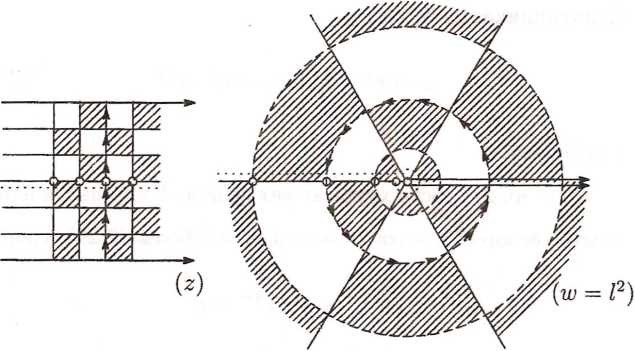
\includegraphics[width=8cm]{Zurag/34.jpg}
    \captionof{figure}{}
        \label{}
\end{center}
$z=x+iy$ ба $w=\rho e^{i\theta}$ гэвэл (\ref{7.32}) ёсоор $w=e^z$ буулгалтыг туйлын координатад 
\begin{eqnarray}
\rho =e^x, \quad \theta =y
\end{eqnarray}
дүрстэй бичье. Эндээс энэ буулгалтыг $\{y=y_0\}$ шулууныг \\ $\{\theta =y_0\}$ цацрагт, харин $x=x_0$, $0<y<2\pi $ хэрчмийг цэгээр цоорхойт тойрогт тус тус буулгана (зураг 25). $\{0<y<2\pi \}$ зурвас бодит хагас тэнхлэгийн дагуу хагалбар бүхий $W$ хавтгайд буух нь тогтоогдлоо. 2 дахин нарийн $\{0<y<\pi\}$ зурвас $\{\im z>0\}$ дээд хагас хавтгайд бууна.

\subsection{Тригонометр функцүүд.} \index{Тригонометр функцүүд.} Эйлерийн томьёоноос дурын $x$-бүхний хувьд $e^{ix}=\cos x+i\sin x$, $e^{-ix}=\cos x-i\sin x$ ба эндээс
$$\cos x=  \frac{e^{ix}+e^{-ix}}{2}, \qquad \sin x  =\frac{e^{ix}-e^{-ix}}{2i}.$$

Энэ томьёонуудыг комплекс хавтгай дээр $\forall z\in\mathbb{C}$-ийн хувьд тодорхойлогдох косинус ба синусийн голоморф үргэлжлэл байдлаар 
\begin{eqnarray} \label{7.34}
\cos z =\frac{e^{iz}+e^{-iz}}{2}, \qquad \sin z=\frac{e^{iz}-e^{-iz}}{2i}
\end{eqnarray}
ашиглаж болно. 

(Баруун гар дахь илэрхийллүүдээс $\mathbb{C}$ дээр голоморф байх нь илэрхий).

Эдгээр функц илтгэгч функцээр тодорхойлогдох тул түүний бүхий л чанар хадгалагдана. Хоёулаа үет функц, үндсэн үе нь $2\pi $ (илтгэгч функц $2\pi i$ үетэй (\ref{7.34}) томьёонд $z$-ийн үржигдэхүүн нь $i$ байх учраас). Косинус-тэгш, синус-сондгой функц. Эдгээр функцүүдийн хувьд уламжлалын ердийн томьёонууд хүчинтэй:
$$(\cos z)'=i\frac{e^{iz}-e^{-iz}}{2}=-\sin z$$
энэчлэн $(\sin z)'=\cos z$. Мөн тригонометр
$$\cos^2 z+\sin^2 z=1, \qquad \cos z=\sin\left(z+\frac{\pi}{2}\right)$$
шүтэлцлүүд, нийлбэрийн теорем гэх мэтчилэн хүчинтэй хэвээр байхыг (\ref{7.34}) томьёоноос төвөггүй тогтоогдоно.

$\forall z\in\mathbb{C}$-ийн хувьд
\begin{eqnarray} \label{7.35}
\ch z=\frac{e^z+e^{-z}}{2}, \qquad \sh z=\frac{e^z-e^{-z}}{2i}
\end{eqnarray}
гэж тодорхойлогдох гипербол функцүүд тригонометр функцүүдтэй нягт холбоотой. 

Энэ холбоо (\ref{7.34}) ба (\ref{7.35}) томьёонуудыг жиших замаар гарах 
\begin{eqnarray} \label{7.36}
\begin{split}
    &\ch z=\cos iz, \qquad \sh z=-i\sin iz \\
    &\cos z=\ch iz, \qquad \sin z=-\sh iz
\end{split}
\end{eqnarray}
шүтэлцлүүдээр илэрхийлэгдэнэ.

Нийлбэрийн теорем ба (\ref{7.36}) томьёонууд ашиглан бичвэл 
\begin{align*}
    &\cos z =\cos(x+iy)=\cos x\ch y-i\sin x\sh y\\
    &\sin z= \sin(x+iy)=\sin x\ch y-i\sh y \cos x
\end{align*}
бөгөөд эндээс
\begin{eqnarray}
\begin{split}
    &|\cos z|=\sqrt{\cos^2x+\sh ^2y} \\
    &|\sin z|=\sqrt{\sin^2x+\sh^2 y}
\end{split}
\end{eqnarray}
байна. (Энд $\cos^2x+\sin^2x=1$, $\ch^2y-\sh^2y=1$ адилтгалууд ашиглав.) Энэ томьёонууд косинус ба синус функцүүдийн модулийн гадаргуу (рельеф) байгуулах боломж олгоно.\\
Жишээ болгож косинусын рельефийг\index{Рельеф косинусын} зураг 35 дээр дүрслэв. \\
\begin{center}
    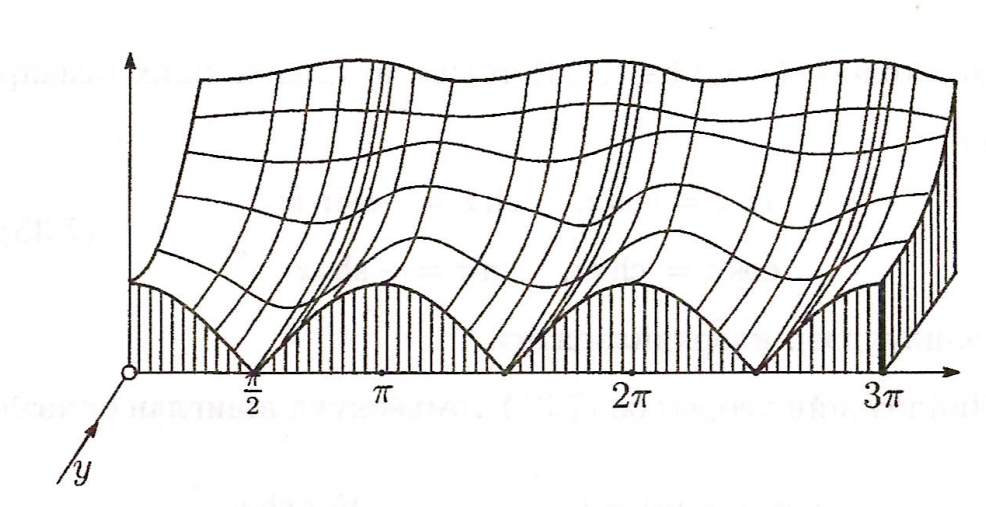
\includegraphics[width=8cm]{Zurag/35.PNG}
    \captionof{figure}{}
        \label{}
\end{center}

$w=\sin z$ функц дээд хагас хавтгайд байх \\ $D=\left\{-\dfrac{\pi}{2}<x<\dfrac{\pi}{2}, \quad y=0\right\}$-хагас зурвас мужийг хэрхэн буулгахтай танилцъя. Энэ буулгалт бидний урьдын танил хялбар
$$z_1=iz,\quad z_2=e^{z_1}, \quad z_3=\frac{z_2}{i}, \quad w=\dfrac{1}{2}\left(z_3+\frac{1}{z_3}\right)$$
буулгалтууд болон задарна. 

Иймд $w=\sin z$ функц $D$ мужийг дээд хагас хавтгайд нэг хуудаст (бөгөөд конформ) буулгана. 

Ингэхдээ $\{x=x_0, \quad 0<y<\infty\}$ цацрагийг $\pm 1$ цэгт фокус бүхий гиперболын хэсэгт,  $х\left\{-\dfrac{\pi}{2}<x<\dfrac{\pi}{2}, \quad y=y_0\right\}$ хэрчмийг мөн тийм фокусууд бүхий эллипсийн хэсэгт бууна. Зураг $36$-аас харахад \\
\begin{center}
    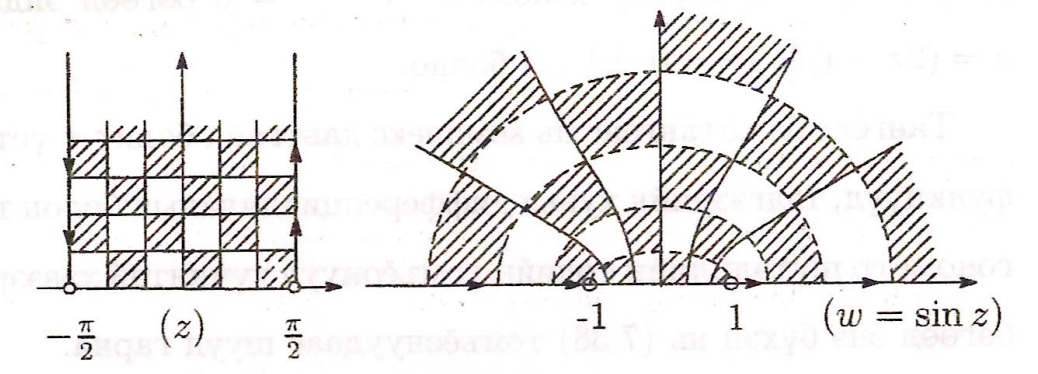
\includegraphics[width=9cm]{Zurag/36.PNG}
    \captionof{figure}{}
        \label{}
\end{center}
хагас зурвас мужийн босоо хилүүд $w=\sin z$-функцээр бодит тэнхлэгийн модуль 1-ээс их хэсэгт буух нь тодорхой байна.

Тангенс ба котангенс функцүүд комплекс аргументийн хувьд 
\begin{eqnarray}
\tan z=\frac{\sin z}{\cos z}, \qquad \cot z=\frac{\cos z}{\sin z}
\end{eqnarray}
томьёонуудаар тодорхойлогдоно. Эдгээр нь итгэгч функцээр рационал байдалтай
\begin{eqnarray} \label{7.38}
\tan z=-i\frac{e^{iz}-e^{-iz}}{e^{iz}+e^{-iz}}, \quad \cot z=i \frac{e^{iz}+e^{-iz}}{e^{iz}-e^{-iz}}
\end{eqnarray}
илэрхийлэгдэнэ. Эдгээр функцүүд (\ref{7.38}) томьёонуудын хуваарийн $0$-тэй тэнцэх цэгүүд (тэдгээр дээр хүртвэр нь $0$-ээс ялгаатай)-ээс бусад нийт $\mathbb{C}$ дээр голоморф байна. 

Жишээ нь $\tan z$ функцийн тийм цэгүүдийг олъё. Тэдгээр дээр $\cos z=0$, өөрөөр хэлбэл $e^{iz}+e^{-iz}=0$ бөгөөд эндээс $z=(2z-1)\dfrac{\pi}{2}$, $(n=0,\pm 1, \ldots)$ болно.

Тангенс ба котангенс нь комплекс хавтгайд бодит $\pi$ үетэй функцүүд, тэдгээрийн хувьд дифференциалчлалын болон тригонометр шүтэлцлийн ердийн томьёонууд хүчинтэй хэвээрээ бөгөөд энэ бүхэн нь (\ref{7.38}) томьёонуудаас шууд гарна.

Тангенс функцийг бидний танил хялбар
\begin{eqnarray} \label{7.39}
z_1=2iz, \quad z_2=e^{z_1}, \quad w=-i\frac{z_2-1}{z_2+1}
\end{eqnarray}
функцүүдийн тусламжтайгаар түүний буулгалтыг харуулъя. $w=\tan z$ функц $\left\{-\dfrac{\pi}{4}<x<\dfrac{\pi}{4}\right\}$ зурвасыг (\ref{7.39}) ёсоор нэгж дугуйд $1$ хуудаст бөгөөд конформ буулгана.

Энэ буулгалтаар $\{x=x_0\}$ шулуунууд $\pm 1$ цэгүүдийн дайрах тойргийн нумд харин  $\left\{-\dfrac{\pi}{4}<x<\dfrac{\pi}{4}, \quad y=y_0\right\}$хэрчмүүд түүний төгсгөлийн цэгүүдийг тэгш хэмтэйгээр агуулах тойргийн нумд хувиргана.

Зарим жишээ авч үзье.
\begin{exm}
Дээд хагас $P=\{z:\im z>0\}$ хавтгайг өөрт нь $w(0)=1$,$w(i)=2i$ нөхцөлтэйгөөр буулга.
\end{exm}
\begin{sol}
2 дахь нөхцөлөөс харахад $-i$ цэг $2i$-тэй тэгш хэмтэй $-2i$ цэгт буух тул (\ref{7.17}) ёсоор 
$$\frac{w-1}{w-2i}\cdot \frac{-2i-2i}{-2i-1}=\frac{z-0}{z-i}\cdot \frac{-i-i}{-i-0}$$ буюу $w=-2\cdot \dfrac{2z+1}{z-12}.$
\end{sol}
\begin{exm}
Дээд хагас $P=\{z:\im z>0\}$хавтгайг нэгж $K=\{w:|w|<1\}$ дугуйд $w(i)=0$, $\arg  w'(i)=-\dfrac{\pi}{2}$ нөхцөлтэй буулга.
\end{exm}
\begin{sol}
(\ref{7.18}) томьёогоор 
$$w=e^{i\theta}\cdot \frac{z-i}{z+i}$$
бөгөөд $$w'(z)=e^{i\theta}\cdot \dfrac{2i}{(z+i)^2}, \quad w'(i)=e^{i\theta} \left(-\dfrac{i}{2}\right)$$ болж $\arg  w'(i)=-\dfrac{\pi}{2}$ нөхцөлөөс $\theta -\dfrac{\pi}{2}=-\dfrac{\pi}{2}$ буюу $\theta= 0$ тул $w=\dfrac{z-i}{z+i}.$
\end{sol}
\begin{exm}
$K=\{z:|z|<1\}$ тойргийг $\overline{K}=\{w:|w-i|<1\}$ тойрогт шилжүүлэх $w$ буулгалтыг $w(0)=\dfrac{i}{2}$ ба $w(1)=0$ байхаар ол.
\end{exm}
\begin{sol}
(\ref{7.13}) томьёо ёсоор $w=\dfrac{i}{2}$ цэгт тэгш хэмт $w^*$ цэг олбол
$$w^*=i+\frac{1}{\overline{\frac{i}{2}-i}}=-i$$
бөгөөд эндээс $w(\infty)=-i$ улмаар (\ref{7.17}) ёсоор
$$\frac{w-\frac{i}{2}}{w-0}\cdot \frac{-i-0}{-i-\frac{i}{2}}=\frac{z-0}{z-1}\cdot \frac{\infty -1}{\infty -0}.$$ болж 
$w=\dfrac{i-iz}{z+2}.$
\end{sol}
\begin{exm}
$D=\{z:|z|<1\}\cap \{z:|z-1|>1\}$ мужийг дээд хагас $P=\{w:\im w>0\}$ хавтгайд буулга.
\end{exm}
\begin{sol}
Тойргийн нумуудаар зааглагдсан саран $D$ мужийг дээд хагас $P$ хавтгайд буулгахын тулд эхлээд түүнийг бутархай шугаман функцээр төгсгөлгүй сектор мужид буулгана.  

Үүний тулд
$\left.\begin{array}{c}
     |z|=1  \\
     |z-1|=1
\end{array}\right\}$ системээс
$$z_1=\frac{1}{2}+\frac{\sqrt{3}}{2}i, \quad z_2=\frac{1}{2}-\frac{\sqrt{3}}{2}i$$
цэгүүдийг олж $z_2\rightarrow 0$, $z_1\rightarrow \infty$ байх бутархай шугаман $w_1$ буулгалт байгуулбал:
$$w_1=\frac{z-z_2}{z-z_1}=\frac{2z-1+\sqrt{3i}}{2z-1-\sqrt{3i}}$$
\begin{align*}
    &w_1(0)=\frac{-1+\sqrt{3i}}{-1-\sqrt{3i}}=-\frac{1}{2}-\frac{\sqrt{3}}{2}i\\
    &w_1(1)=\frac{2-1+\sqrt{3i}}{2-1-\sqrt{3i}}=-\frac{1}{2}+\frac{\sqrt{3}}{2}i
\end{align*}
цэгүүдийн дайрах цацрагууд $D$-ийн хилд буух тул эдгээрийн хоорондох өнцөг $(w_1(0)^{\wedge}w_1(1))=\dfrac{2\pi}{3}$ байх учраас $w_2=e^{-i\frac{2\pi}{3}}w_1$ болно.

Эндээс $w=w_2^{\frac{3}{2}}$ болж бидний эрж байгаа буулгалт:
$$w=-\left(\frac{2z-1+\sqrt{3}i}{2z-1-\sqrt{3}i}\right)^{\frac{3}{2}}$$
\end{sol}
\begin{center}
    \textbf{Дасгал}
\end{center}
\begin{enumerate}
    \item $K=\{z:|z|<1\}$ дугуйг дээд хагас $P=\{w:\im w>0\}$ хавтгайд буулгах бутархай шугаман функцийг $w(-1)=\infty$, $w(1)=0$, $w(i)=1$ нөхцөлөөр ол.
    \item Нэгж $K=\{z:|z|<1\}$ дугуйг өөрт нь өөрөөр хэлбэл
$\overline{K}=\{w:|w|<1\}$ буулгах функцийг $w\left(\frac{1}{2}\right)$, $\arg  w'\left(\frac{1}{2}\right)=\dfrac{\pi}{2}$ нөхцөлөөр ол.
\item $\gamma=\{z:|z-i|=3\}$ тойргийн хувьд $2+i$ цэгтэй тэгш
хэмтэй цэгийг ол.
\item Дээд хагас $P=\{z:\im z>0\}$ хавтгайг нэгж $K=\{w:|w|<1\}$ дугуйд $w(2i)=0$, $\arg  w'(2i)=0$ нөхцөлөөр буулга.
\item 	Дараах хоёр өнцөгт (саран) мужийг дээд хагас хавтгайд буулга:
\begin{enumerate}
    \item [a)] $D_1=\{z:|z|<1\}\cap \{z:|z-i|<1\}$
     \item [b)] $D_2=\{z:|z|>1\}\cap \{z:|z-i|<1\}$
\end{enumerate}
\end{enumerate}
\chapter{Голоморф функц ба төгсгөлгүй үржвэр
}
\section{Үндсэн ойлголтууд}
\begin{dfn}
$u_k\in\mathbb{C}(k=1,2,3,\ldots)$ байг. 
$$P_n=(1+u_1)(1+u_2)(1+u_3)\cdot \ldots \cdot (1+u_n)$$ гэж тодорхойлъё.
\begin{enumerate} \label{8.1}
    \item [a)] Хэрэв $\exists \lim\limits_{n\rightarrow \infty} P_n=P\in \mathbb{C}$ ба $P\neq 0$ бол 
    \begin{eqnarray}
     P=\prod\limits_{k=1}^\infty (1+u_k)
    \end{eqnarray}  төгсгөлгүй үржвэр \index{Төгсгөлгүй үржвэр} нийллээ гэж үздэг.
 \item [б)] Хэрэв дээрх хязгаар оршдоггүй эсвэл $0$ байвал сарниж байна гэж үздэг.
  \item [в)] Хэрэв $\exists \tilde{P}=\prod\limits_{k=1}^\infty (1+|u_k|)\in\mathbb{R}\setminus \{0\}$ байвал абсолют нийлдэг төгсгөлгүй үржвэр\index{Абсолют нийлдэг төгсгөлгүй үржвэр} гэж үздэг.
  \item [г)] Төгсгөлгүй үржвэр нийлдэг боловч абсолют нийлэхгүй
  $$\left( \text{жишээ нь} \left(1+\frac{1}{2}\right)\left(1-\frac{1}{2}\right) \left(1+\frac{1}{3}\right) \left(1-\frac{1}{4}\right)\cdots \right)$$
  бол нөхцөлт нийлдэг үржвэр гэдэг.
\end{enumerate}
\end{dfn}
\textbf{Дасгал 1}. Дараах үржвэр ба цуваануудын нийлэлт сарнилт нь ижил байна. 
\begin{eqnarray}
 \prod\limits_{k=1}^\infty (1+|u_k|)
\end{eqnarray}
\begin{eqnarray}
 \sum\limits_{k=1}^\infty \ln (1+|u_k|)
\end{eqnarray}
ба 
\begin{eqnarray} \label{8.4}
 \sum\limits_{k=1}^\infty |u_k|
\end{eqnarray}
\begin{cor}
(\ref{8.1})-ийн абсолют нийлэлтийг шинжихдээ (\ref{8.4}) цувааг судалж болно.

Тоон цуваанаас функцэн цуваанд шилжих алхмыг үржвэрт бас хэрэглэж болно. Тухайлбал:
\end{cor}
\begin{thm}
$u_k(z)\in H(D)(k=1,2,3,\ldots)$ байг. $\forall k\in\mathbb{N}:|u_k(z)|\leq a_k$ байдаг ба $a_1+a_2+\cdots +a_k+\cdots$ цуваа нийлдэг байг. Тэгвэл  
$$\exists P(z)=\prod\limits_{k=1}^\infty (1+u_k(z))\in H(D)$$ байна.
\end{thm}
\begin{prf}
$a_1+a_2+\cdots +a_n+\cdots$ эерэг тоон цуваа нийлэх тул $\forall z\in D$ хувьд жиших шинжүүр ёсоор $$|u_1(z)|+|u_2(z)|+\cdots +|u_k(z)|+\cdots$$
цуваа нийлнэ. Иймд $P(z)$ утга оршино.

Одоо $$P(z,n)=(1+u_1(z))(1+u_2(z)\cdot \ldots \cdot(1+u_n(z))$$
$\tilde{P}=\prod\limits_{k=1}^\infty (1+a_k)$ ба $\tilde{P}(n)=\prod\limits_{k=1}^n (1+a_k)$ гэж тэмдэглэе.
\begin{equation}
    \tag{$*$} \label{8*}
    \begin{split}
        &|P(z,n)|=|1+u_1(z)|\cdot |1+u_2(z)|\cdot \ldots \cdot |1+u_n(z)|\leq \\
        &\leq (1+|u_1(z)|)(1+|u_2(z)|)\cdot \ldots \cdot (1+|u_n(z)|)\leq \tilde{P}(n)
    \end{split}
\end{equation}
\begin{equation}
    \tag{$**$} \label{8**}
    \begin{split}
    &\left|\frac{P(z)}{P(z,n)}-1\right|=\lim\limits_{k\rightarrow\infty}\left|\frac{P(z,n+k)}{P(z,n)}-1\right|=\\
        &\leq\lim\limits_{k\rightarrow\infty}(|u_{n+1}(z)|+ |u_{n+2}(z)|+ \cdots + |u_{n+k}(z)|+\cdots \\
        &\cdots +|u_{n+1}(z)\cdot u_{n+2}(z)\cdot \ldots \cdot u_{n+k}(z)|)\leq\\
        &\leq \lim\limits_{k\rightarrow \infty} (a_{n+1}+a_{n+2}+\cdots +a_{n+k}+a_{n+1}\cdot a_{n+2}+\cdots\\
        &\cdots +a_{n+1}\cdot a_{n+2}\cdot \ldots \cdot a_{n+k})= \\
        &=\lim\limits_{k\rightarrow \infty}\left(\frac{\tilde{P}(n+k)}{\tilde{P}(n)}-1\right) =\frac{\tilde{P}}{\tilde{P}(n)}-1\Rightarrow \\
        &\Rightarrow \left|\frac{P(z)}{P(z,n)}-1\right|\leq \frac{\tilde{P}}{\tilde{P}(n)}-1
    \end{split}
\end{equation}
болно. (\ref{8*}), (\ref{8**}) ашиглавал
\begin{align*}
    |P(z)-P(z,n)|&=|P(z,n)|\cdot \left|\frac{P(z)}{P(z,n)}-1\right| \leq \\
    &\leq \tilde{P}(n)\cdot \left(\frac{\tilde{P}}{\tilde{P}(n)}-1\right) =\tilde{P}-\tilde{P}(n)\xrightarrow[n\rightarrow\infty]{} 0
\end{align*}
учир $P(z,n)$ функцэн дараалал $P(z)$-рүү жигд нийлж байна. Иймд Вейерштрассын теорем ёсоор $P(z)\in H(D)$ болж батлагдав.
\hfill $\blacksquare$\end{prf}
\section{Төгсгөлгүй үржвэр ба бүхэл функц}
$a_1,a_2,\ldots ,a_n,\ldots$ тэгээс ялгаатай гишүүдтэй комплекс тоон дарааллын хувьд 
\begin{eqnarray} \label{8.5}
 |a_k|\leq |a_{k+1}| \quad \text{ба} \quad |a_k|\rightarrow +\infty
\end{eqnarray} байг. 
\begin{thm}
\textbf{(Вейерштрасс).}  Тэгвэл $p\in\mathbb{N}$ үед
\begin{eqnarray} \label{8.6}
 G(z)=z^{p-1}\cdot \prod\limits_{k=1}^\infty \left(1-\frac{z}{a_k}\right)\cdot e^{\frac{z}{a_k}+\frac{1}{2}\left(\frac{z}{a_k}\right)^2+\cdots +\frac{1}{k-1}\cdot \left(\frac{z}{a_k}\right)^{k-1}}
\end{eqnarray}
функц
\begin{enumerate}
    \item [a)] Бүхэл функц байна (өөрөөр хэлбэл $G(z)\in H(G))$
      \item [б)] $G(a_k)=0 \quad (\forall k).$
     \item [в)] $p-1$ нь $z=0$ цэг $G(z)=0$ тэгшитгэлийн шийд болох эрэмбэ нь байна.
     \item [г)] Өөр тэглэгч цэг $G(z)$ функцэд байхгүй.
\end{enumerate}
\end{thm}
Энэ теоремын баталгааг орхив.\\
Харин $exp$ үржигдэхүүн нь төгсгөлгүй үржвэрийн нийлэлтийг хангахад шаарддагийг тэмдэглэе. Теоремын урвуу нь дараах хэлбэрээр батлагдсан байдаг.
\begin{thm}
$\forall f(z)\in H(\mathbb{C})$ бүхэл функц авч үзье. Түүний тэглэгч цэгийн тоо төгсгөлгүй $a_1,a_2, \ldots, a_k,\ldots$  дараалал үүсгэдэг бол
$$f(z)=e^{H(z)}\cdot z^{p-1}\prod\limits_{k=1}^\infty \left(1-\frac{z}{a_k}\right) e^{\frac{z}{a_k}+\frac{1}{2}\left(\frac{z}{a_k}\right)^2+\cdots +\frac{1}{n-1}\cdot \left(\frac{z}{a_kk}\right)^{n-1}} $$ байна. Үүнийг Вейерштрассын томьёо \index{Вейерштрассын томьёо} гэнэ. Энд $p\in\mathbb{N}$ ба $H(z)$ ямар нэг бүхэл функц байна. 
\end{thm}
\begin{exm}
$f(z)=\sin z$ гэж авъя. Тэглэгч цэгүүд нь $z=k\pi $ учир
\begin{align*}
    \sin z&=e^{H(z)}\cdot z\cdot \prod\limits_{k=-\infty}^{+\infty} \left(1-\frac{z}{k\pi}\right) e^{\frac{z}{k\pi}+\frac{1}{2}\left(\frac{z}{k\pi}\right)^2+\cdots +\frac{1}{n-1}\cdot \left(\frac{z}{k\pi}\right)^{n-1}}=\\
    &=e^{\tilde{H}(z)}\cdot z\cdot \prod\limits_{k=1}^{\infty} \left(1-\frac{z}{k\pi}\right)\left(1-\frac{z}{-k\pi}\right)=\\
    &=e^{\tilde{H}(z)}\cdot z\cdot \prod\limits_{k=1}^{\infty} \left(1-\frac{z^2}{k^2\pi^2}\right)
\end{align*}
(энд $k$ ба $-k$ гишүүдээр нь бүлэглэснээр абсолют нийлдэг үржвэр үүссэн тул ехр үржигдэхүүнүүдийн илтгэгчийг $H(z)$ дээр нэмж $\tilde{H}(z)$-р тэмдэглэв).

$\tilde{H}(z)$  функцийг олж тогтооход дээрх теорем тус болохгүй. Тухайн тохиолдолд
$$\cot (z)=\frac{1}{z}+\sum\limits_{k=1}^\infty \frac{2z}{z^2-k^2\pi^2}$$
гэж байдгийг шууд ашиглаж $(\ln\sin z)'$ уламжлалыг судалснаар $H(z)=1$ болохыг тогтоож болно. Үүнийг дасгал болгон ажиллаарай. Ийнхүү
$$\sin z=z\cdot \prod\limits_{k=1}^\infty\left(1-\frac{z^2}{k^2\pi^2}\right)$$
\end{exm}
\begin{center}
  \textbf{  Дасгал}
\end{center}
\begin{enumerate}
    \item $e^z-1=e^{\frac{z}{2}}\cdot z\cdot \prod\limits_{k=1}^\infty \left(1+\dfrac{z^2}{4\pi^2k^2}\right)$
    \item $\cos z=\prod\limits_{k=1}^\infty \left(1-\dfrac{4z^2}{\pi^2(2k-1)^2}\right);$
    \item $\dfrac{2\sin iz}{e^{2z}-1}=e^{-z+\frac{\pi}{2}i}$ 
\end{enumerate} байдгийг тус тус харуул.
\section{Мерорморф функц\index{Мерорморф функц}}
$\mathbb{C}$ хавтгайд туйлын цэгүүдээс өөр онцгой цэггүй функцийг мероморф функц гэж тодорхойлдог. \\
\textbf{Дасгал.} Мероморф функцийн туйлын цэгүүд нь төгсгөлтэй хязгаарын цэгтэй байж болохгүй.\\
\textbf{Заавар.} Тийм хязгаарын цэг оршдог гэвэл тэр нь онцгойрлын цэг болно. Гэтэл мероморф функцийн тодорхойлолт ёсоор уг цэг туйлын онцгой цэг байна. Энэ цэг дээрх Лораны цувааг ерөнхий хуваарьт оруулж харвал ямар зөрчил үүсэхийг ол.\\
\begin{cor}
Мероморф функц нь төгсгөлтэй эсвэл (\ref{8.5}) нөхцөлийг хангасан төгсгөлгүй олон туйлын цэгүүдтэй байна.
\end{cor}
$f(z)$ нь мероморф функц бол $G(z)$ бүхэл функцийг эсвэл олон гишүүнт (\ref{8.6}) томьёогоор байгуулахдаа $f(z)$-н туйлын цэг бүр нь яг тэр эрэмбээрээр $G(z)$-н тэглэгч цэг байхаар байгуулж болно. Энэ үед
\begin{eqnarray}
 G_1(z)=f(z)\cdot G(z)
\end{eqnarray}
бүхэл функц болно. Ийнхүү:

\begin{thm}
Аливаа мероморф функц нь хоёр бүхэл функцийн ноогдвор хэлбэрт тавигдана.
\end{thm}
\section{Аналитик үргэлжлэлийн тодорхойлолт} \index{Аналитик үргэлжлэл}
Морерын теорем ёсоор хоёр голоморф функц тодорхойлогдох мужуудынхаа огтлолцол $D=D_1\cap D_2$; $int D\neq 0$ дээр ижил байвал $D_1\cup D_2$ муж дээр голоморф функц тодорхойлдог.

 Мөн $D_1$ муж дээрх голоморф функцийг $D_2\setminus D$ муж руу өргөтгөх өөр функц байхгүй нь нэг утгын теоремоор батлагдсан. Ингэж өгөгдсөн функцийн голоморф чанарыг алдуулалгүй тодорхойлох мужийг нь өргөтгөж байгааг аналитик үргэлжлэл хийгдэж байна гэдэг.
 \begin{center}
     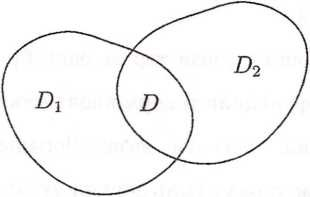
\includegraphics[width=5cm]{Zurag/37.jpg}
 \captionof{figure}{}
        \label{ref hiih ner}
 \end{center}
\begin{exm}
$y=\sin x$ функц $\mathbb{R}$-дээр тодорхойлогдсон байг. Үүний хувьд функц байх нь $\mathbb{C}$ дээрх аналитик үргэлжлэл байх нь 
$$\sin x=\sum\limits_{k=0}^\infty (-1)^k\cdot \frac{x^{2k+1}}{(2k+1)!} \quad (x\in\mathbb{R})$$
тэнцэтгэлээс харагдаж байна.
\end{exm}
\begin{exm}
$$f(z)=1+z+z^2+\cdots \in H(|z|<1)$$ бол $g(z)=\dfrac{1}{1-z}\in H(\mathbb{C}\setminus \{1\})$ нь аналитик үргэлжлэл гэдгийг батал.
\end{exm}
Эндээс харвал ямар нэг $D$ мужид голоморф функц өгөгдсөнөөр түүнийг аналитик үргэлжлүүлсээр цааш өргөжүүлэх боломжгүй болсон үед үүсэж байгаа объектыг бүрэн аналитик функц гэнэ. Бүрэн аналитик функц өөрийн өчүүхэн хэсгээрээ ганц утгатай тодорхойлогддог.

\section{Бүрэн аналитик функц тодорхойлох Вейерштрассын арга }\index{Вейерштрассын арга}
$f\in H(D)$ байх функц өгөгдөв. Дурын $z_1\in D$ цэгийг авснаар энэ цэгийн орчинд өгөгдсөн функц
\begin{eqnarray} \label{8.8}
 f(z)=\sum\limits_{n=0}^\infty a_n(1)(z-z_1)^n
\end{eqnarray}
Тейлорын цуваанд задарна. Энэ цувааны нийлэлтийн радиус $R_1$ хязгааргүй бол функц бүхэл функц болон өргөтгөгдөнө. Харин (\ref{8.8}) цувааны нийлэлтийн радиус төгсгөлөг бол уг дугуйгаас $z_2(z_2\neq z_1)$ цэг сонгон авч
\begin{eqnarray}
 f(z)=\sum\limits_{n=0}^\infty a_n(2)(z-z_2)^n
\end{eqnarray}
цуваанд задалъя.

Хэрэв $R_2>R_1-|z_2-z_1|$ бол функц анхны дугуйн $z_2-z_1$ радиус векторын дагуу аналитик үргэлжлэл зохиогдоно. Эсрэг тохиолдолд уг чиглэлийн дагуу үргэлжлэхгүй байна. Одоо (\ref{8.8}) элементийг бүх чиглэлийн дагуу үргэлжлүүлсэн гэвэл цааш үргэлжлэхгүй $$\left (z_k; \quad \sum\limits_{n=0}^\infty a_n(k)(z-z_k)^n\right)$$ элементүүдээс тогтсон бүтэц үүснэ. Энэ бүтцийн бүрэн аналитик функц Вейерштрассын аргаар өгөгдлөө гэдэг. Дугуйгаар дамжин үргэлжилсээр нэг эгшинд дугуй өмнө таарч байсан дугуйтай огтлолцох нь бий. Энэ үед элементүүдийн зэрэгт цувааны утга ерөнхий хэсэгтээ таарах эсвэл эс таарах тохиолдол үүснэ.
\begin{center}
    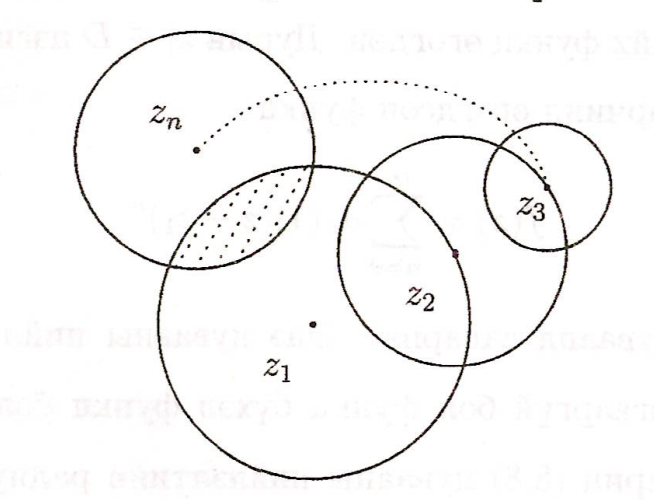
\includegraphics[width=6cm]{Zurag/38.PNG}
    \captionof{figure}{}
        \label{}
\end{center}
\section{Бүрэн аналитик функц тодорхойлох \\
Риманы арга \index{Риманы арга}
}
Риманы арга нь $\mathbb{C}$ хавтгайн оронд Риманы гэж нэрлэгдэх тусгай гадаргуунууд авч үзсэнээр олон утгат бүрэн аналитик функцийг нэг утгатай функцийн тодорхойлолтод нийцүүлдэг.
\begin{exm}
$w=\sqrt{z}$ буулгалт нь $w_1=\sqrt{\rho}\cdot e^{i\frac{\varphi}{2}}$; $w_2=\sqrt{p}e^{i\left(\frac{\varphi}{2}+\pi \right)}$ хоёр мөчир функцэд задардгийг өмнө үзсэн. $\mathbb{C}$ хавтгайг сөрөг хагас тэнхлэгийн дагуу хайчилсан мужийг $D$ гэе. Дээрх мөчир функцүүд нь $D$ мужийг харгалзан $\mathbb{C}$ хавтгайн баруун ба зүүн хагас хавтгайд буулгана. ($E_1$ ба $E_2$ гэж эдгээрийг тэмдэглэе). Одоо $D$ мужийг 2 ширхэг авч зурагт үзүүлсэн наалтыг хийе:\\
\begin{center}
    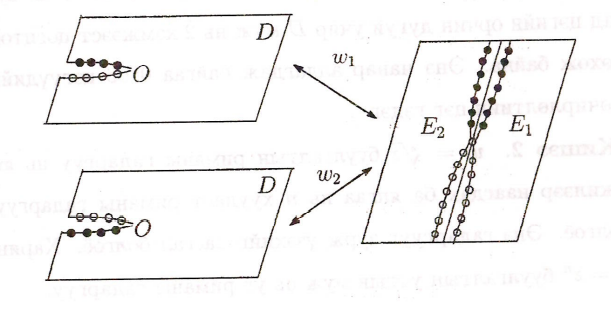
\includegraphics[width=8cm]{Zurag/39.PNG}
\end{center}
\begin{center}
    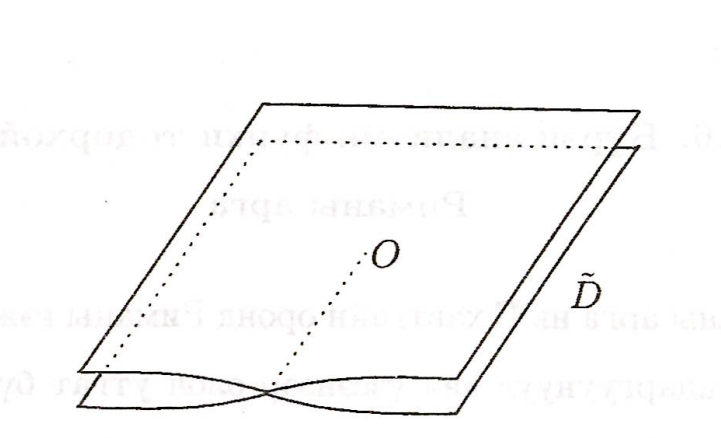
\includegraphics[width=6cm]{Zurag/39.2.PNG}
    \captionof{figure}{}
        \label{}
\end{center}
Хар цэгээр тэмдэглэсэн ирмэгүүдийг хооронд нь, цагаанаар тэмдэглэснийг нь хооронд нь нааснаар $\tilde{D}$ өвөрмөц гадаргуу үүснэ (Жич: Ердийн цаасыг ингэж наах нь боломжгүй, 2-р наалтын үед $\tilde{D}$) өөрөө өөрийгөө огтолж байгаа мэт боловч ингэж огтлохгүйгээр топологи утгаар наасан гэж сэтгэдэг).

Ийнхүү $w=\sqrt{z}$ буулгалт нь  $\tilde{D}\rightarrow E=E_1\cup E_2$ харилцан нэг утгатай функц болон хувирав. $D$ мужийг хуудас гэж нэрлэх ба $\tilde{D}$ мужийг 2 хуудаст гэдэг. $0;\infty \in\tilde{D}$ бусад цэгийн орчин дугуй учир $\tilde{D}$ муж нь 2 хэмжээст цогцтой дөхөж байна. Энэ чанар алдагдаж байгаа $0,\infty$ цэгүүдийг мөчирлөлтийн цэг гэдэг.
\end{exm}
\begin{exm}
$w=\sqrt[n]{z}$ буулгалтын риманы гадаргуу \index{Риманы гадаргуу} нь яг ижлээр наагдах ба ялгаа нь $n$ хуудаст риманы гадаргуу болгоё. Энэ гадаргууг зурж үзэхийг дасгал болгоё. Харин $w=z^n$ буулгалтын утгын муж нь уг риманы гадаргуу.
\end{exm}
\begin{exm}
$w=\ln z$ буулгалт нь төгсгөлгүй хуудаст Риманы гадаргуутай байдаг.
$w_k=\ln \rho +i(\varphi +2\pi k)(k\in\mathbb{Z})$ мөчир нь $D$ мужийг
$$E_k=\{w:2\pi k -\pi \leq \im w<2\pi k +\pi\}$$ зурваст буулгана гэдгийг өмнө үзсэн.
\begin{center}
    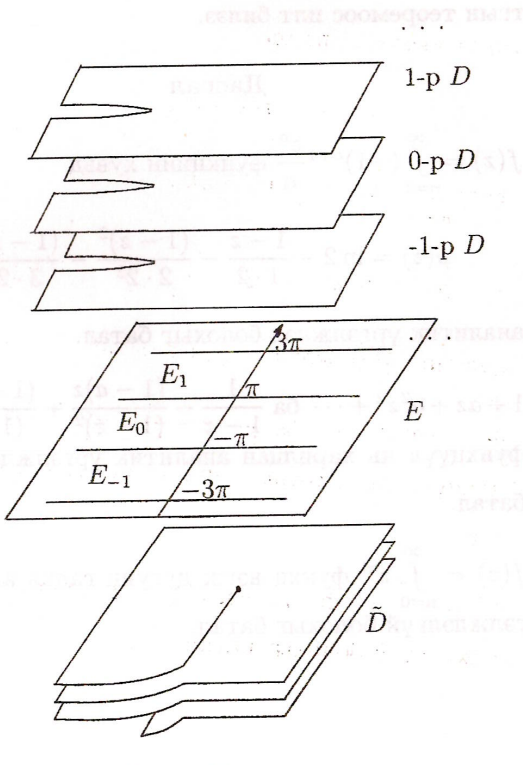
\includegraphics[width=5cm]{Zurag/40.PNG}
    \captionof{figure}{}
        \label{}
\end{center}
Иймээс хязгааргүй олон $D$ мужийг өмнөх жишээний зарчмаар төгсгөлгүй наасан гэж сэтгэвэл $\tilde{D}$ риманы гадаргуу нь үүснэ.

Эцэст нь дурдахад бүрэн аналитик функцийн энэхүү хоёр байгуулалт нь яг ижил, нэг нь нөгөөдөө шилждэг гэдэг нь нэг утгын теоремоос илт билээ.
\end{exm}
\begin{center}
   \textbf{ Дасгал}
\end{center}
\begin{enumerate}
    \item [4.] $f(z)=\bint\limits_{n=1}^\infty (-1)^{n+1}\dfrac{z^n}{n}$ функцийн хувьд 
    $$g(z)=\ln 2-\frac{1-z}{1\cdot 2}-\frac{(1-z)^2}{2\cdot 2^2}-\frac{(1-z)^3}{3\cdot 2^3}\cdot \ldots$$
    аналитик үргэлжлэл болохыг батал.
    \item [5.] $$1+az+a^2z^2+\cdots \quad \text{ба} \quad \frac{1}{1-z}-\frac{(1-a)^z}{(1-z)^2}+\frac{(1-a)^2z^2}{(1-z)^3}-\cdots$$
    функцүүд нь харилцан аналитик үргэлжлэл болдгийг батал.
\item [6.] $f(z)=\bint\limits_{n=0}^\infty z^{n!}$ функц нэгж дугуйн гадна аналитик үргэлжлэлгүй болохыг батал.
\end{enumerate}
\chapter{Геометр зарчмууд}
Энэ бүлэгт голоморф функцийн ерөнхий топологи шинжүүдийг үзүүлдэг геометр онолын зарчмуудыг оруулав.